We will utilize the following diagrammatic simplification
\begin{center}
	\boxed{\begin{tikzpicture}[scale=.4]
		\draw (6,2)--(7,1)--(7,0);
		\draw (8,2)--(7,1);
		\node at (6,2.5){$\scriptstyle 1$};
		\node at (7,2.5){$\scriptstyle \dots$};
		\node at (8,2.5){$\scriptstyle n$};
		
		\draw (11,.5)--(12,1.5)--(12,2.5);
		\draw (13,.5)--(12,1.5);
		\node at (11,0){$\scriptstyle 1$};
		\node at (12,0){$\scriptstyle \dots$};
		\node at (13,0){$\scriptstyle n$};
		\end{tikzpicture}}
\end{center}
to represent labeled directed graphs resulting from iterated grafting of \product and \coproduct \ in the left comb order
\begin{center}
	\boxed{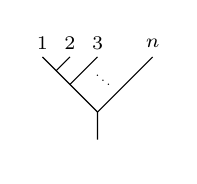
\begin{tikzpicture}[scale=.35]		
		\node at (-2.15,-.25){};
		\node at (-2.15,3.25){};
		
		\node at (-2,3.5){$\scriptstyle 1$};
		\node at (-1,3.5){$\scriptstyle 2$};
		\node at (0,3.5){$\scriptstyle 3$};
		\node at (2,3.5){$\scriptstyle n$};
		
		\draw (-2,3)--(0,1);
		\draw (2,3)--(0,1)--(0,0);
		\draw (0,3)--(-1,2);
		\draw (-1,3)--(-1.5,2.5);
		\draw (.2,2.3) node[scale= 0.5] {$\ddots$};
		\end{tikzpicture}
		\qquad 
		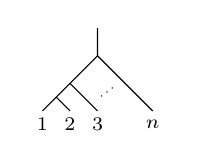
\begin{tikzpicture}[scale=.35]	
		
		\node at (-2,-3.5){$\scriptstyle 1$};
		\node at (-1,-3.5){$\scriptstyle 2$};
		\node at (0,-3.5){$\scriptstyle 3$};
		\node at (2,-3.5){$\scriptstyle n$};
		
		\draw (-2,-3)--(0,-1);
		\draw (2,-3)--(0,-1)--(0,0);
		\draw (0,-3)--(-1,-2);
		\draw (-1,-3)--(-1.5,-2.5);
		\draw (.2,-2.3) node[scale= 0.5, rotate = 75] {$\ddots$};
		\end{tikzpicture}}
\end{center}

A \textit{surjection-like graph} is either the $(1,0)$-graph \counit\ or for $n > 1$ a $(1, n)$-graph of the form 
\begin{center}
\boxed{\begin{tikzpicture}[scale=.4]
	\node at (5,8){$\scriptstyle 1$};
	\draw (3,5.5)--(5,6.5)--(5,7.5);
	\draw (7,5.5)--(5,6.5);
	\node at (3,5){$\scriptstyle 1$};
	\node at (5,5){\,$\scriptstyle \dots$};
	\node at (7,5){$\scriptstyle r+d$};
	
	\node at (5,4){$\vdots$};
	
	\node at (3,-.5){$\scriptstyle 1$};
	\draw (2,2)--(3,1)--(3,0);
	\draw (4,2)--(3,1);
	\node at (2,2.5){$\scriptstyle 1$};
	\node at (3,2.5){$\scriptstyle \dots$};
	\node at (4,2.5){$\scriptstyle k_1$};
	
	\node at (5,1){\ $\cdots$};
	
	\node at (7,-.5){$\scriptstyle r$};
	\draw (6,2)--(7,1)--(7,0);
	\draw (8,2)--(7,1);
	\node at (6,2.5){$\scriptstyle 1$};
	\node at (7,2.5){$\scriptstyle \dots$};
	\node at (8,2.5){$\scriptstyle k_r$};
	\end{tikzpicture}}
\end{center}
containing no internal vertices and such that for each $i = 1, \dots, r$ the induced map 
\begin{equation*}
\{1, \dots, k_i\} \to \{1, \dots, r+d\}
\end{equation*}
is order preserving.